% Created 2017-01-30 Mon 14:06
% Intended LaTeX compiler: pdflatex
\documentclass[bigger]{beamer}
\usepackage[utf8]{inputenc}
\usepackage[T1]{fontenc}
\usepackage{graphicx}
\usepackage{grffile}
\usepackage{longtable}
\usepackage{wrapfig}
\usepackage{rotating}
\usepackage[normalem]{ulem}
\usepackage{amsmath}
\usepackage{textcomp}
\usepackage{amssymb}
\usepackage{capt-of}
\usepackage{hyperref}
\mode<beamer>{\useinnertheme{rounded}\usecolortheme{rose}\usecolortheme{dolphin}\setbeamertemplate{navigation symbols}{}\setbeamertemplate{footline}[frame number]{}}
\mode<beamer>{\usepackage{amsmath,amsthm,amssymb,mathtools,tikz,multirow}\usepackage{ae,aecompl}}
\let\oldframe\frame\renewcommand\frame[1][allowframebreaks]{\oldframe[#1]}
\setbeamertemplate{frametitle continuation}[from second]
\newcommand{\backupbegin}{\newcounter{framenumberappendix}   \setcounter{framenumberappendix}{\value{framenumber}}}
\newcommand{\backupend}{ \addtocounter{framenumberappendix}{-\value{framenumber}}  \addtocounter{framenumber}{\value{framenumberappendix}}}
\usetheme{default}
\author{Ole Jann* and Christoph Schottmüller** \linebreak \vspace*{0.3cm}\linebreak\scriptsize{*Nuffield College, Oxford\linebreak **University of Copenhagen}}
\date{}
\title{An informational theory of privacy}
\hypersetup{
 pdfauthor={Ole Jann* and Christoph Schottmüller** \linebreak \vspace*{0.3cm}\linebreak\scriptsize{*Nuffield College, Oxford\linebreak **University of Copenhagen}},
 pdftitle={An informational theory of privacy},
 pdfkeywords={},
 pdfsubject={},
 pdfcreator={Emacs 25.1.1 (Org mode 9.0.3)}, 
 pdflang={English}}
\begin{document}

\maketitle
\begin{frame}{Outline}
\tableofcontents
\end{frame}



\section{Introduction}
\label{sec:org4472673}

\begin{frame}[label={sec:org5e7ecd5}]{Privacy is a hot topic}
\begin{itemize}
\item government surveillance
\item business surveillance
\begin{itemize}
\item e-business: data as side product of any transaction
\item loyalty cards
\end{itemize}
\item voluntary provision of personal data (facebook, twitter, mobile phone)
\item micro targeting in election campaigns
\end{itemize}

\pause

\vspace*{0.5cm}
\begin{center}
What is at stake? trade-offs? mechanisms?
\end{center}
\end{frame}


\begin{frame}[label={sec:org9f30475}]{What is privacy (in this paper)?}
\begin{itemize}
\item ability to take actions without being observed, and having interactions with others confined to the intended recipients
\item (many other definitions)
\item privacy \(\subset\) asymmetric information
\end{itemize}

\pause

\vspace*{0.3cm}
\begin{center}
\begin{large}
Is there an economic rationale for privacy?
\end{large}
\end{center}
\end{frame}


\begin{frame}[label={sec:org25f7efd}]{Economics of privacy: Chicago school (Stigler 80, Posner 81)}
\begin{itemize}
\item privacy = asymmetric information
\item asymmetric information = inefficiency (Akerlof, Mirrlees etc.)
\end{itemize}

\(\Rightarrow\) privacy = inefficiency 
\end{frame}

\begin{frame}[label={sec:org49d6a19}]{Popular debate: "Nothing to hide"}
\begin{itemize}
\item reiterated by Google, facebook, NSA etc.
\begin{itemize}
\item If you have nothing to hide, you do not need privacy.
\item If you have something to hide, you should not do it.
\end{itemize}
\end{itemize}
\end{frame}

\begin{frame}[label={sec:orge999e65}]{This paper}
\begin{itemize}
\item our model:
\begin{itemize}
\item information is not perfect (correlation: statistical discrimination as in Phelps 72, Arrow 73)
\item privacy affects behavior
\end{itemize}
\item main result: privacy can be efficient even when considering \emph{informational effects only}
\item other results:
\begin{itemize}
\item lack of privacy changes behavior in one direction ("chilling effects")
\item effectiveness of privacy intrusion is easily overstated
\item privacy is redistributive

\item mandating privacy might be necessary to avoid unraveling
\end{itemize}
\end{itemize}
\end{frame}



\section{Model}
\label{sec:orgf7d2a89}

\begin{frame}[label={sec:org7e6a6a6}]{A simple story}
\begin{itemize}
\item Alice thinks drugs should be legalized and wants to write on her facebook profile about that.
\item She is also looking for a job.
\item Employers do not want to hire drug users.
\item positive correlation between stand on legalization (\(\theta_i\)) and drug use (\(\tau_i\))
\item two cases: The employer can see what Alice does online, or not.
\end{itemize}
\end{frame}



\begin{frame}[label={sec:org6fccddb}]{Model I}
\begin{itemize}
\item \(n\) individuals
\item individual \(i\) has type \((\theta_i,\tau_i)\)
\begin{itemize}
\item \(\theta_i\sim \mathcal{N}(0,1)\)
\item \(\tau_i\) positively correlated with \(\theta_i\) \linebreak (formally: distribution of \(\tau_{\text{i}}\) at \(\theta_{\text{i}}\)' fosd distribution at \(\theta_{\text{i}}\)''<\(\theta\)')
\end{itemize}
\end{itemize}

\begin{center}
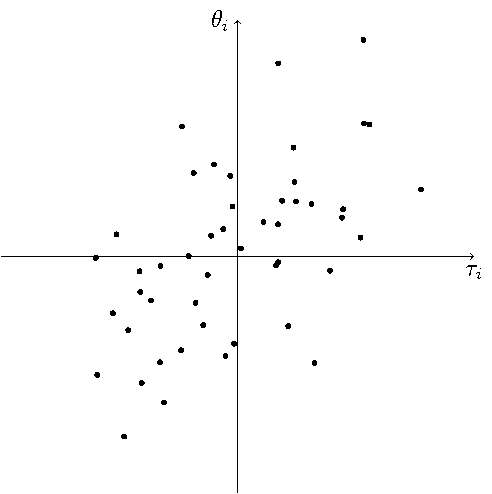
\includegraphics[scale=0.6]{scatter}
\end{center}
\end{frame}

\begin{frame}[label={sec:org386ad2b}]{Model II}
\begin{enumerate}
\item information aggregation stage
\begin{itemize}
\item \(i\) observes \((\theta_i,\tau_i)\)
\item \(i\) chooses \(p_i\in\{0,1\}\)
\item policy \(p\in\{0,1\}\) is implemented with probability \(q(m/n)\) where \(m/n\) is fraction of individuals choosing \(p_i=1\)
\item \(q'>0\) and \(q\) point symmetric around 0.5
\item payoff for \(i\): \(p\theta_i\)
\end{itemize}
\item interaction stage
\begin{itemize}
\item opposing player (OP) chooses action A (aggressive) or M (mild) against \(i\)
\item payoff OP: A gives \(\tau_i\), M gives 0
\item payoff \(i\): A gives \(-\delta(\tau_i)\), M gives 0
\item \(\delta\) weakly increasing
\end{itemize}
\end{enumerate}

no privacy: OP knows \(p_i\)

privacy: OP has only prior
\end{frame}

\section{Results}
\label{sec:org783dea5}

\begin{frame}[label={sec:org5edcb1f}]{Results: Chilling effect}
\begin{itemize}
\item individuals use cutoff strategies: \(p_i=1\) iff \(\theta_i\geq t(\tau_i)\)
\end{itemize}

\begin{block}{Proposition (Chilling effect)}
With privacy \(t^p(\tau_i)=0\). \linebreak Without privacy \(t^{np}(\tau_i)\geq0\) and \(t^{np}(\tau_i)\) is increasing.
\end{block}

\begin{itemize}
\item without privacy individuals with \(\theta_i\in [0,t(\tau_i))\) change their behavior ("are chilled")
\item without privacy OP plays M against \(p_i=0\) and A against \(p_i=1\) \linebreak (if privacy affects OP behavior and pure strategy equilibrium)
\end{itemize}
\end{frame}

\begin{frame}[label={sec:org79d4e99}]{Equilibrium without privacy}
\begin{center}
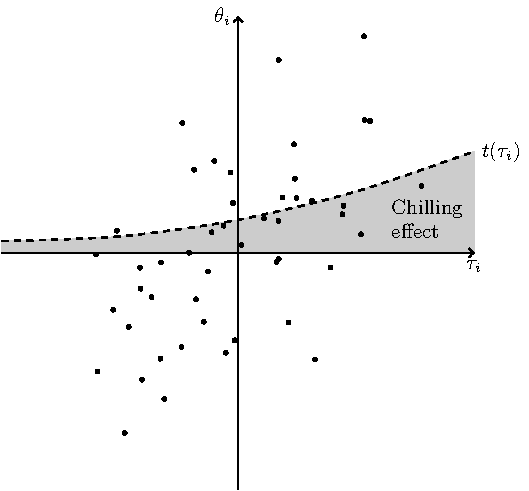
\includegraphics[scale=0.95]{graphchilling.pdf}
\end{center}
\end{frame}

\begin{frame}[label={sec:org73c079e}]{Welfare results}
\begin{block}{Lemma (Consumer surplus)}
Expected consumer surplus in the information aggregation stage is maximal at the privacy cutoff \(t^p(\tau_i)=0\).
\end{block}
\pause

\begin{itemize}
\item welfare includes OP payoff (OP might loose from privacy)
\end{itemize}

\begin{theorem}[Welfare]
Let \(\delta'>0\).

For \(n\) sufficiently large, expected consumer surplus is higher under privacy and OP payoff is the same under privacy and no privacy.

Let the disutility of A be \(-r\delta(\tau_i)\). For \(r\) sufficiently high, consumer surplus is higher under privacy and OP payoff is the same under privacy and no privacy.
\end{theorem}
\end{frame}

\begin{frame}[label={sec:org49941e1}]{Privacy is redistributive}
\begin{itemize}
\item individuals with \(\theta_i<0\) loose from privacy
\item individuals that are chilled \(\theta_i\in[0, t^{np}(\tau_i)\) gain a bit from privacy
\item individuals with \(\theta_i>t^{np}(\tau_i)\) gain double from privacy (decision, OP interaction)
\end{itemize}
\end{frame}


\begin{frame}[label={sec:orgb79935e}]{Surveillance performs worse than expected}
\begin{itemize}
\item seems as eliminating privacy could give OP huge benefit
\item but: behavior change (chilling) might reduce correlation between \(p_i\) and \(\tau_i\)
\item technical assumption (TA): \(\mathbb{E}[\tau_i|\theta_i=0]\geq 0\) \linebreak (if OP knew \(\theta_i\) and \(\theta_i\geq0\), A would be best response)
\end{itemize}

\begin{block}{Lemma}
Assume TA. \linebreak OP's payoff without privacy is lower if individuals use \(t^{np}\) than if they used \(t^p=0\).
\end{block}
\end{frame}

\begin{frame}[label={sec:orgf83e285}]{Surveillance performs worse than expected}
\begin{center}
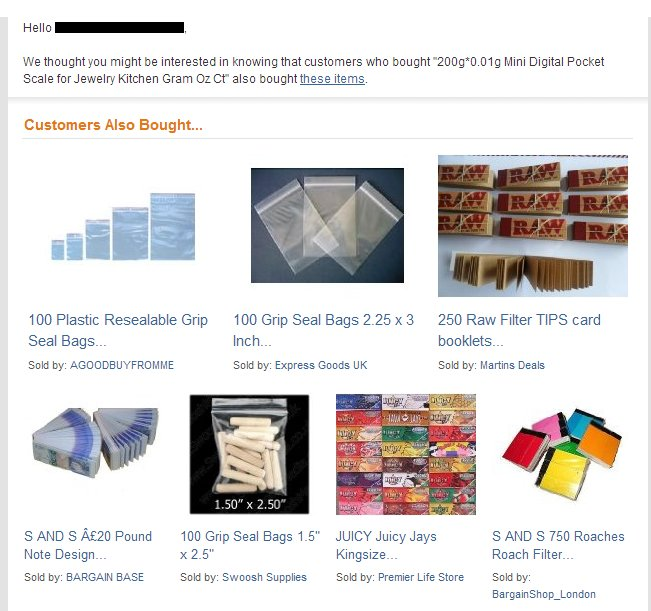
\includegraphics[scale=0.4]{example1}
\end{center}
\end{frame}

\begin{frame}[label={sec:orgcdf0799}]{More stuff in the paper I}
\begin{itemize}
\item Extension: privacy as opt in
\begin{itemize}
\item individuals can choose whether to keep \(p_i\) private or not
\item multiple equilibria
\item privacy is not a robust equilibrium: unraveling
\end{itemize}
\item Extension: endogenous information aggregation mechanism \(q\)
\begin{itemize}
\item \(q\) is chosen to maximize consumer surplus taking (no) privacy into account
\end{itemize}
\item Extension: defensive action
\begin{itemize}
\item Alice can hire a lawyer to help her with the employer
\item \(i\) can take costly defensive action that reduces the disutility of A and lowers the payoff of OP (regardless of his action)
\item equilibria where OP is strictly better off with privacy
\end{itemize}
\end{itemize}
\end{frame}
\begin{frame}[label={sec:org6c561d7}]{More stuff in the paper II}
Alternative setups for stage 1:
\begin{itemize}
\item private decision
\begin{itemize}
\item stage 1: no information aggregation, i.e. no externalities from \(p_j\) on \(i\)
\item additional result: privacy is welfare optimal if correlation between \(\theta_i\) and \(\tau_i\) is not too high
\end{itemize}
\item state matching
\begin{itemize}
\item stage 1: payoff of each \(i\) is \(p\theta\) where \(\theta\) is an unknown state and each \(i\) has a noisy signal \(\theta_i\)
\item same results but privacy makes every \(i\) better off as chilling inhibits efficient information aggregation
\end{itemize}
\end{itemize}
\end{frame}
\section{Applications}
\label{sec:org63b8543}
\begin{frame}[label={sec:org777f5c5}]{Discussion: When is privacy bad?}
\begin{itemize}
\item biased information aggregation \(q\)
\begin{itemize}
\item chilling can counteract bias
\end{itemize}
\item externalities: 
\begin{itemize}
\item insider trading
\item video surveillance to deter vandalism might prevent other crimes
\end{itemize}
\end{itemize}
\end{frame}

\begin{frame}[label={sec:org31064fd}]{Application: Chilling effects in election polls}
\begin{itemize}
\item secret ballot: election is private and influences decision
\item poll: less private (interviewer), less influential \linebreak \(\rightarrow\) chilling effects
\item Bischoping and Schuman (1992)
\end{itemize}
\end{frame}

\begin{frame}[label={sec:org1be534e}]{Application: Credit scoring}
repayment probability (\(\tau_{i}\)) is not directly observable
\begin{itemize}
\item Consider two characteristics (\(\theta_{i}\)) that are predictive of \(\tau_{i}\): education and music taste
\item Low education and a preference for rap music predict low repayment probability.
\item There is a chilling effect in both cases, but in the first we might consider it desirable!?
\item Should the bank be allowed to use data on music taste? (``Equal Credit Opportunity Act'' outlaws ``redlining'' in the US)
\item blacklist vs. whitelist
\end{itemize}
\end{frame}

\begin{frame}[label={sec:org1623462}]{Application: Working in committees}
\begin{itemize}
\item committee is debating two policies (e.g. raise interest rates or not)
\item debate and vote can either be in secret or in public
\item correlation between policy preference \(\theta_{i}\) and competence \(\tau_{i}\)
\item members worry about being perceived as incompetent; advocate less radical positions
\item Fed is forced to publish minutes of FOMC meetings since 1993; \linebreak increase in conformity and a decrease of disagreement with the chairman (Meade and Stasavage 2008)
\item Thomas Hoenig, President of the Kansas City Fed: ``The tape has had some chilling effect on our discussions. I see a lot more people reading their statements.''
\end{itemize}
\end{frame}


\section{Conclusion}
\label{sec:org96eb9c8}
\begin{frame}[label={sec:orgac86ba8}]{Conclusion}
\begin{itemize}
\item we give a simple model to understand privacy from the perspective of information economics
\begin{itemize}
\item no privacy leads to chilling effects
\item privacy can be welfare optimal
\item privacy is redistributive (similar to freedom of speech, Friedman 72)
\end{itemize}
\item the model leads to interesting policy questions
\begin{itemize}
\item blacklist vs. whitelist
\item how open should government be?
\item mandate vs. option of privacy
\item which kind of data should be accessible by who?
\end{itemize}
\item we identify crucial elements to address these questions (correlation, behavior change, threat potential)
\end{itemize}


\backupbegin
\end{frame}

\begin{frame}[label={sec:org01ea6a8}]{Literature}
\begin{itemize}
\item Chicago school (Stigler 80, Posner 81)
\item statistical discrimination (Phelps 72, Arrow 73)
\item Hirshleifer effect (Hirshleifer 71)
\item intrinsic motivation + image concerns and privacy (Daughety and Reinganum 2010, Ali and Benabou \emph{working paper})
\item equilibrium effects of privacy (Cummings et al. \emph{working paper})
\item many papers in specific IO settings 
\begin{itemize}
\item dynamic pricing if purchase history is known/unknown 
\begin{itemize}
\item sophisticated vs. naive consumers
\end{itemize}
\item differentiated good competition with known/unknown location
\end{itemize}
\item survey: Acquisti et al. JEL 2015
\end{itemize}
\end{frame}

\section{Presentation}
\label{sec:org390a3d0}

\begin{frame}[label={sec:org98d39e5}]{Christoph Schottmüller}
\begin{center}
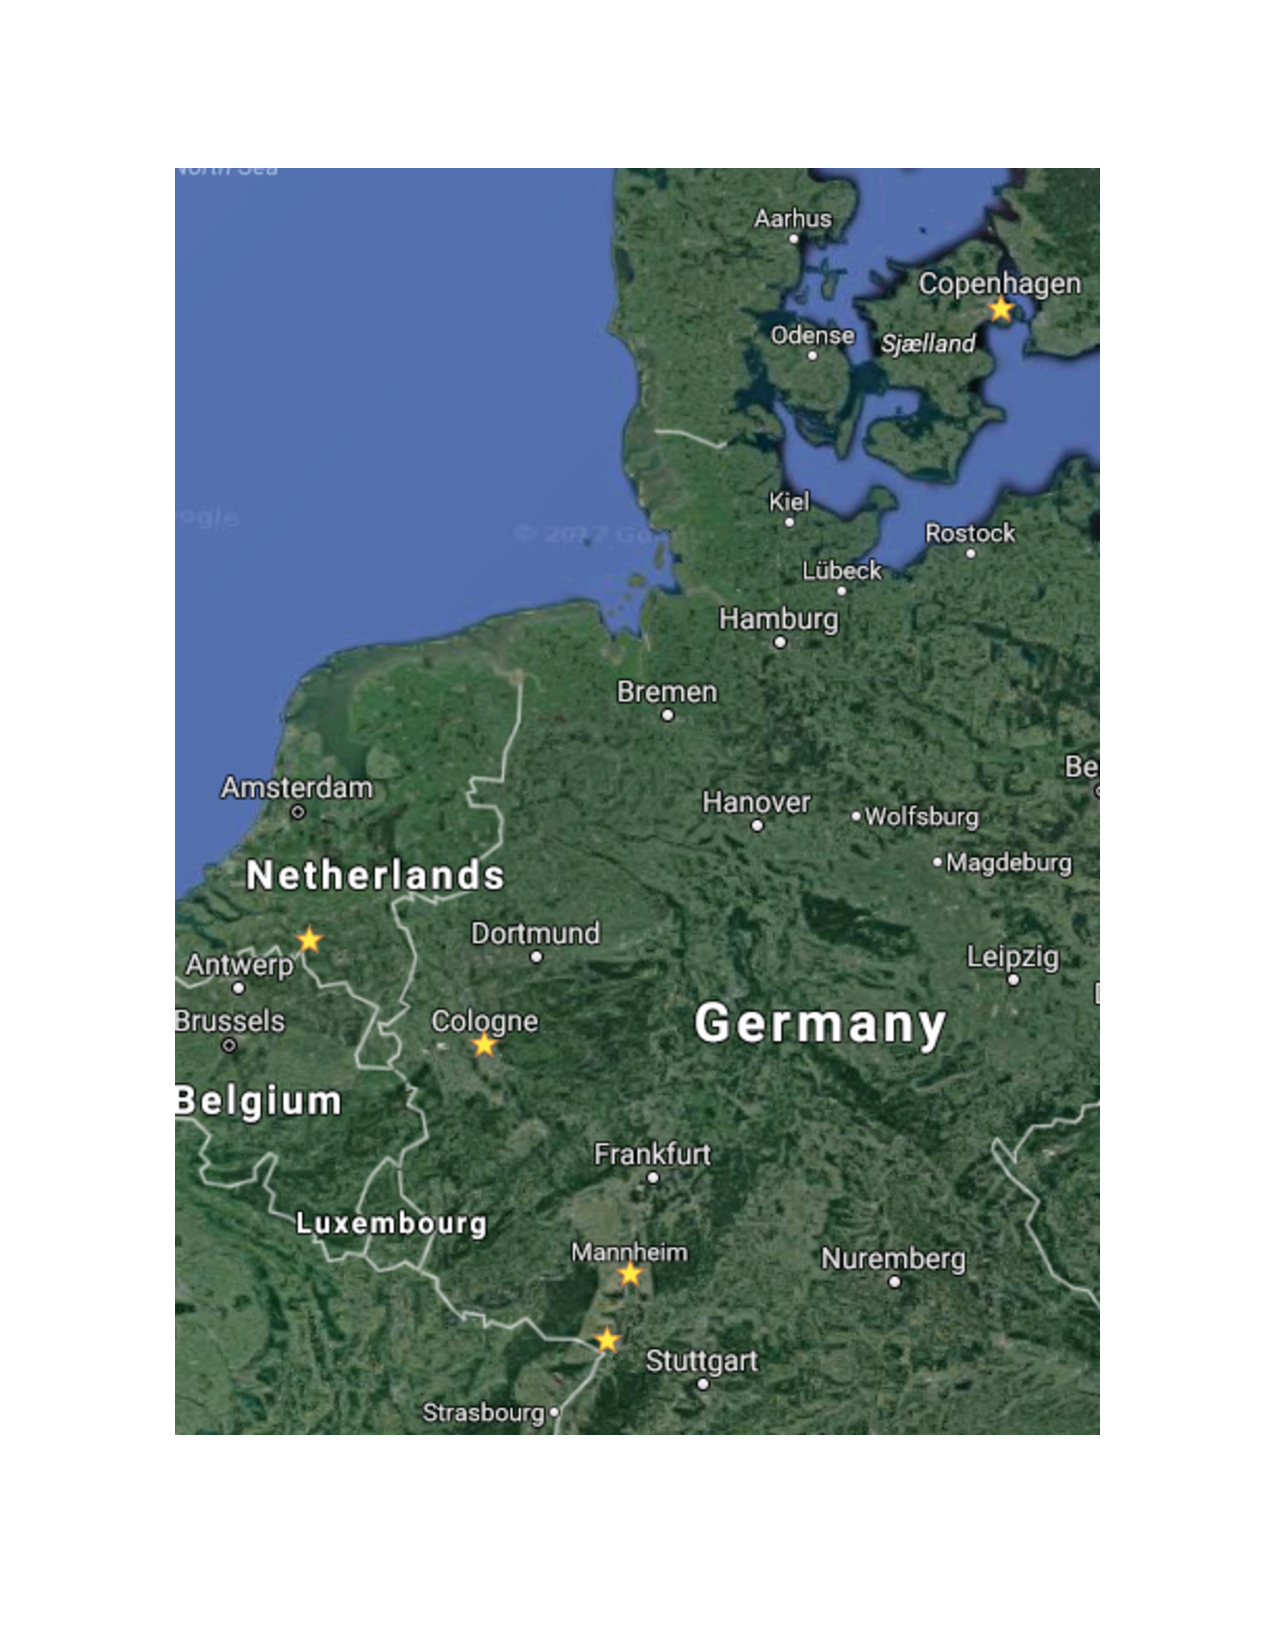
\includegraphics[scale=0.35]{map2}
\end{center}
\end{frame}

\begin{frame}[label={sec:orgf8692b2}]{Research}
\begin{itemize}
\item past:
\begin{itemize}
\item contract theory: principal agent problems, (health) insurance
\item IO: procurement, pricing
\end{itemize}

\item ongoing/future:
\begin{itemize}
\item privacy and surveillance
\item dynamic advice and reputation
\item IO of data driven markets (e.g. internet search)
\item political polarization and echo chambers
\item information design
\end{itemize}
\item methods: theory + \ldots{}
\end{itemize}
\end{frame}

\begin{frame}[label={sec:orgc226fc5}]{Teaching}
\begin{itemize}
\item past/ongoing:
\begin{itemize}
\item courses:
\begin{itemize}
\item game theory
\item mechanism design
\item health insurance (MSc Public Health)
\end{itemize}
\item \href{./gt2016.html}{how}?
\end{itemize}
\end{itemize}

\pause

\begin{itemize}
\item possibilities for future: 
\begin{itemize}
\item standard microeconomics courses
\item auction theory
\item economics of the internet
\item (topics in) information economics
\item (topics in) industrial organization (and incentive regulation)
\end{itemize}
\end{itemize}
\end{frame}

\begin{frame}[label={sec:org5a72ce3}]{Cologne and Christoph}
\begin{itemize}
\item overlapping research interests 
\begin{itemize}
\item design questions
\item (applied) game theory
\item advice and reputation
\item digital markets
\item incentive regulation and IO
\item (applied) contract theory
\item (applied) mechanism design
\end{itemize}

\item complementarities in teaching
\item institutional fit:
\begin{itemize}
\item Faculty division: Microeconomics, Institutions and Markets
\item Key research profile area: Design and Behavior
\item CSEB 
\begin{itemize}
\item Design and Behavior
\end{itemize}
\end{itemize}
\end{itemize}
\end{frame}

\begin{frame}[label={sec:org29280ce}]{From a project description}
"Many markets are plagued by moral hazard and adverse selection problems, and so require trust in order to function effectively. In this project, we study how advice and reputation promote trust [\ldots{}] We start with the observation that traders with limited information often rely on expert advice. E.g., many retail investors seek financial advice, which however may be compromised by a conflict of interest with the advisor."\par 
(CSEB, Design and Behavior, Engineering Trust in Markets: Advice and Reputation)

\backupend
\end{frame}
\end{document}